\documentclass[11pt,letterpaper]{article}
\usepackage[T1]{fontenc}
\usepackage{lmodern,microtype}
\usepackage[margin=.85in,headheight=15pt]{geometry}
\usepackage{xcolor,booktabs,longtable,array,tabularx,enumitem,amsmath,graphicx,listings,tikz,fancyhdr,titlesec,hyperref,xurl}
\usetikzlibrary{arrows.meta,positioning,fit,shapes.geometric}
\definecolor{navy}{HTML}{16314D}\definecolor{teal}{HTML}{087F83}\definecolor{pale}{HTML}{EDF4F8}\definecolor{muted}{HTML}{536579}
\hypersetup{colorlinks=true,linkcolor=navy,urlcolor=teal,pdftitle={Security Architecture Assessment}}
\titleformat{\section}{\Large\bfseries\color{navy}}{\thesection}{.7em}{}
\titleformat{\subsection}{\large\bfseries\color{teal}}{\thesubsection}{.7em}{}
\pagestyle{fancy}\fancyhf{}\fancyhead[L]{\small Agent Harness Engineering}\fancyhead[R]{\small Technical study / v1.0}\fancyfoot[R]{\thepage}
\setlength{\parindent}{0pt}\setlength{\parskip}{5pt}\renewcommand{\arraystretch}{1.18}
\setlist{nosep,leftmargin=*}\newcolumntype{Y}{>{\raggedright\arraybackslash}X}
\newcommand{\src}[1]{\expandafter\nolinkurl\expandafter{\detokenize{#1}}}
\newcommand{\evidence}[1]{\par\smallskip{\small\raggedright\color{muted}\textbf{Source anchor:} #1\par}}
\tikzset{n/.style={draw=navy,rounded corners=2pt,fill=pale,align=center,minimum height=9mm,text width=31mm,font=\small},g/.style={n,draw=teal,fill=teal!7},edge/.style={-Latex,thick,draw=navy},boundary/.style={draw=teal,dashed,rounded corners,inner sep=5pt}}
\lstset{basicstyle=\small\ttfamily,breaklines=true,frame=single,backgroundcolor=\color{pale},columns=fullflexible,showstringspaces=false}
\begin{document}
\begin{titlepage}
\vspace*{1.25in}
{\color{teal}\large AGENT HARNESS COURSE STUDY / 03\par}\vspace{.3in}
{\color{navy}\Huge\bfseries Security Architecture Assessment\par}\vspace{.18in}
{\Large Trust boundaries, injection, authorization, approval and isolation\par}\vspace{.5in}
\rule{\linewidth}{1pt}\par
\textbf{Source:} Richmond Alake's Harness Engineering for AI Agents course export\par
\textbf{Version:} 1.0 \quad 23 November 2026\par
\textbf{Status:} Technical study; not a production authorization\par
\vfill
The model proposes; the harness validates, governs, executes and records.
\end{titlepage}
\tableofcontents\clearpage
\section*{Reading note}
This standalone volume belongs to a six-document study of snapshot \src{8a5edab282632443}. Observed source behavior is distinguished from proposed controls. No live application, external provider or sandbox was independently executed. Test files are contract evidence, not independently verified passing results.

\section{Security architecture assessment}
\subsection{Trust boundaries and threat model}
Assets include user identity, connector credentials, confidential source data, execution rights, stored memories, skill versions, checkpoints and audit evidence. Threat actors include malicious external senders and websites, compromised tools/providers, unauthorized users and insiders. The model and its outputs are untrusted for authorization. A known sender, authenticated MCP session or valid JSON does not imply that content is trusted instructions.
\begin{center}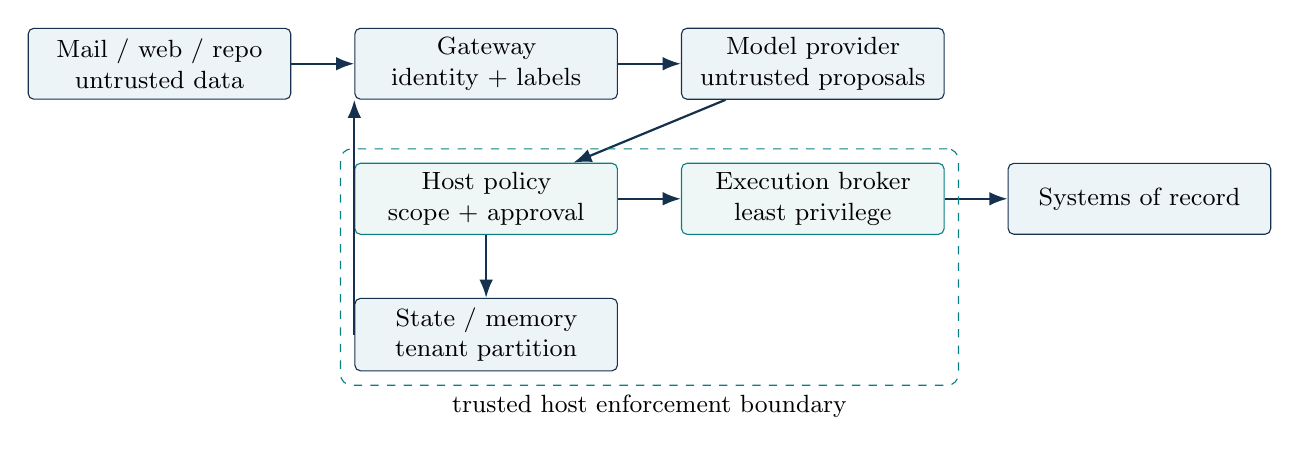
\begin{tikzpicture}[node distance=8mm and 8mm]
\node[n] (ext) {Mail / web / repo\\untrusted data};\node[n,right=of ext] (ing) {Gateway\\identity + labels};\node[n,right=of ing] (llm) {Model provider\\untrusted proposals};
\node[g,below=of ing] (pol) {Host policy\\scope + approval};\node[g,right=of pol] (exec) {Execution broker\\least privilege};\node[n,below=of pol] (mem) {State / memory\\tenant partition};\node[n,right=of exec] (sys) {Systems of record};
\draw[edge](ext)--(ing);\draw[edge](ing)--(llm);\draw[edge](llm)--(pol);\draw[edge](pol)--(exec);\draw[edge](exec)--(sys);\draw[edge](pol)--(mem);\draw[edge](mem.west)-|(ing.south west);
\node[boundary,fit=(pol)(exec)(mem),label=below:{\small trusted host enforcement boundary}] {};
\end{tikzpicture}\end{center}
\textbf{Boundary invariant:} only the authenticated application and broker may make authorization decisions; all adapters recheck the scope of each action. The proposed production boundary is stricter than the course's single-owner educational configuration.
\subsection{Control evidence and risk register}
Ratings are proposed remediation priorities (H high, M medium), not confirmed exploitable vulnerabilities. Verify by negative tests against real deployment configuration before changing the risk rating.
\begin{longtable}{p{.18\linewidth}p{.28\linewidth}p{.30\linewidth}p{.13\linewidth}}\toprule
Threat & Observed course control & Residual risk / required mitigation & Priority \\\midrule\endhead
Prompt injection & Regex tripwire, content wrapper, System One screening, quarantine & Evasion and false negatives; enforce deny rules independently, adversarial evaluation & H \\
Confused deputy & Tool allowlist, validation, recipient checks, effect tiers & Object-level authorization and tenant scope at gateway; no ambient broad credential & H \\
Approval replay & Conditional DRAFTED state update, approved effect log & Bind decision to exact arguments, owner, run, expiry, policy and target version; atomic consumption & H \\
Duplicate external effect & Durable graph, audit and delivery results & Crash after external success before local record; idempotency key, reconciliation, outbox & H \\
Memory poisoning & Scratch promotion, dedupe, quarantine, learning evidence & Dedupe not authenticity; untrusted facts may survive sessions; label and review writes & H \\
Skill poisoning & Candidate gate, held-out checks, replay, version rollback & Gate trial temporarily changes live pointer; isolate candidate namespace, verify rollback target & H \\
Sandbox escape & Fixed local operations; optional E2B governed test & Verify runtime isolation, no host secrets, egress denial, resource and artifact limits & H \\
Cross-tenant exposure & Single-owner practice model; named memory scopes & Tenant and principal separation in DB, cache, checkpoints, logs and retrieval & H \\
Data exfiltration & Safe mode, external recipient warnings & Model-provider transfer, tool outputs and logs; minimize and redact data, egress allowlist & H \\
Resource exhaustion & Bounded loops and research budget & Tenant quotas, atomic reservations, hard deadlines, cancellation & M \\
Supply chain & Requirements files and local/live profiles & Lock hashes, SBOM, signed artifact, scan and isolate dependency upgrades & M \\
\bottomrule\end{longtable}
\subsection{Prompt injection and tool authorization}
The Part 2 policy explicitly calls the regex detector a tripwire rather than a defense. It wraps external content and substitutes closing delimiters, and triage can quarantine instruction-like mail from unknown senders. Part 3 approval code records the course-reported result that the regex caught 31\% of 3,000 successful attacks and none of 203 benign emails. This is source-reported, not independently reproduced. It supports structural controls over classifier-only security. Test indirect injection, paraphrase, multilingual content, forged roles, malicious tool responses, untrusted attachments and persistent memory injection. A classifier outage must not expand permissions.

The observed tiers are automatic (reads and private operations), approval (outward mail/calendar/shared-note changes), and never exposed (e.g., trash, delete, share). Safe mode holds non-owner mail as draft and strips other calendar attendees. A draft and delivered effect are distinct states. Proposed policy applies identity, tenant, tool/version, resource scope, data sensitivity, effect type, recipient, budget and current object state. Unknown tools/identities/resources and malformed input deny by default. MCP is transport, not permission. Restrict discovery and invocation independently; avoid capability escalation through tool chaining.
\evidence{\src{part_2/_shared/runtime/policy.py}; Part 3 \src{approval.py} (TIERS, TRIPWIRE\_FINDING, safe\_mode\_effect), \src{tools.py}, \src{system_one.py}.}
\subsection{Approval, replay and failure semantics}
\begin{center}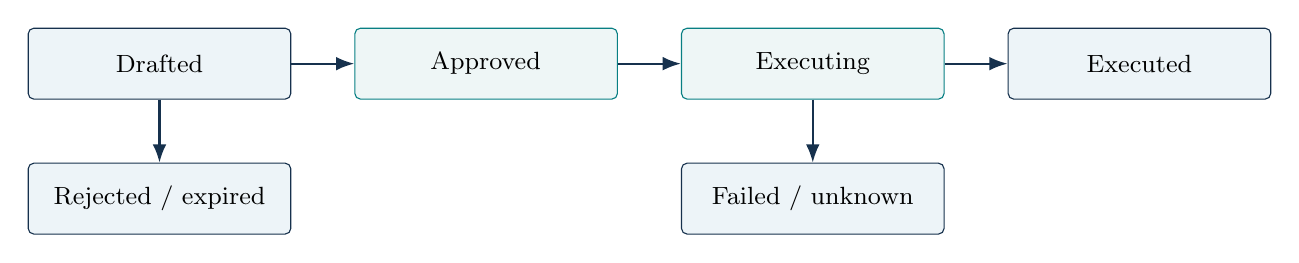
\begin{tikzpicture}[node distance=8mm]
\node[n] (d) {Drafted};\node[g,right=of d] (a) {Approved};\node[g,right=of a] (x) {Executing};\node[n,right=of x] (e) {Executed};\node[n,below=of d] (r) {Rejected / expired};\node[n,below=of x] (f) {Failed / unknown};
\draw[edge](d)--(a);\draw[edge](d)--(r);\draw[edge](a)--(x);\draw[edge](x)--(e);\draw[edge](x)--(f);
\end{tikzpicture}\end{center}
\textit{Figure 1. Proposed durable effect state machine. Executing, expiry and unknown-result reconciliation extend the source's drafted/approved/rejected/executed/failed states.}

Store a canonical action digest over tenant, principal, run, tool version, validated arguments, target version, expiry and policy version. An authenticated human approves that exact digest. On resume, revalidate authorization and object freshness; reject changes. Claim the effect atomically. Call the downstream service with a stable idempotency key where supported. If outcome is uncertain, record UNKNOWN and reconcile via provider read API or manual operator review; never blindly retry an irreversible action. Persist a separate delivery status and compensation record. Rollback does not undo an already sent message.
\evidence{Part 3 \src{approval.py}: decide, executed; \src{agent.py}: human\_review, apply\_effects, resume.}
\subsection{Learning and memory poisoning}
The five named Part 3 checks are real tools, no regression, held-out selection, approval contract and replay. The code temporarily activates a candidate during trials and restores the prior pointer under a gate lock; production must isolate candidate evaluation from serving workers and use transactional version activation. The promotion function requires PASSED, while the activation function can move the pointer to a stored version; verify route-level authorization and restrict rollback to previously approved, compatible versions. A repeated approved workflow indicates utility, not a new security grant. Corrections must not overwrite higher-authority policy or create unreviewed instructions.

Store memory candidates as data with source reference, content hash, confidence, classification, tenant, principal, expiry and review state. Quarantine, validate and promote explicitly. Retrieval filters by identity before ranking; conflicting sources remain separately attributable. Revocation invalidates cache, index and derived procedures; retention includes backups and trace policy. Test poisoning from rejected actions, duplicate evidence, external documents and poisoned evaluation fixtures.
\subsection{Sandbox and secrets}
The Part 1 README describes a fixed-operation local sandbox; the advanced sandbox module has an authorization-policy fixture and a deterministic E2B test double. Distinguish a test double from an isolated live runtime. A production sandbox should use an ephemeral identity, unprivileged user, read-only base filesystem, isolated workspace, restricted mounts, no ambient credentials, default-deny egress, CPU/memory/time/file limits and sanitized artifact return. Validate externally that denied egress and host filesystem access are blocked. Host validation of sandbox results is required even when isolation succeeds. Secrets should come from workload identity/secret manager, not prompts or trace dumps. Disable live tools by default in developer and CI profiles.
\subsection{Suggested acceptance suite}
\begin{longtable}{p{.25\linewidth}p{.66\linewidth}}\toprule
Test & Expected assertion \\\midrule\endhead
Contract & Malformed, oversized and unknown proposal variants deny; no adapter call. \\
Authorization & Wrong actor, cross-scope object and undeclared tool deny; no downstream effect. \\
Approval & Exact validated payload only; denied, expired, modified and consumed approvals cannot execute. \\
Durability & Restart at draft, approval, claim, external success and local commit; no blind retry after unknown result. \\
Memory & Malicious or rejected source never becomes executable instruction; revocation invalidates retrieval and cache. \\
Delegation & Child capability set subset of parent; global budget cannot be exceeded under concurrent calls. \\
Sandbox & Host mount and arbitrary network denied in actual runtime integration tests. \\
Audit & Every effect has linked policy, approval if needed and observed delivery; no secrets in trace. \\
Evaluation & Mandatory evidence present; frozen thresholds pass; independent reviewer records decision. \\
\bottomrule\end{longtable}
\section{Source register and limitations}
\begin{itemize}
\item Richmond Alake, \textit{Harness Engineering for AI Agents}, supplied repository export,\newline snapshot \src{8a5edab282632443}; root README, Part 1--3 READMEs, code paths cited throughout. Workshop: \url{https://www.oreilly.com/live-events/harness-engineering-for-ai-agents/0642572381264}.
\item Target curriculum, README and roadmap, inspected 23 November 2026: \url{https://github.com/Notoriousjayy/agent-engineering-curriculum}.
\item Target documentation library, root README and AI technical-documents directory, inspected 23 November 2026: \url{https://github.com/Notoriousjayy/latex-docs}.
\end{itemize}
All figures are original logical reconstructions or proposed design diagrams; they are not copies of source graphics. Vendor-neutral controls, ADRs, acceptance tests and laboratory extensions are recommendations rather than claims about source implementation. Live dependencies, source test outcomes, provider claims, licensing/publication clearance and deployment configuration require separate validation.
\end{document}
